% 第4節 選択肢集合の困難とネットワーク型選択モデル
%% chapters/behavior_modeling/ch3_choiceset.tex
%% 第3章　選択肢集合
\section{選択肢集合の困難とネットワーク型選択モデル}\label{sec:choiceset}
本節では，選択肢集合の問題と経路非列挙型経路選択モデルについて解説する．
具体的には，選択肢集合の定義の難しさと列挙型モデルの限界を説明した上で，Recursive LogitやDynamic Decision Modelなどの経路非列挙型の経路選択モデルを紹介する．

\subsection{選択肢集合の爆発}
経路選択肢集合は簡単に爆発する．
例えば，$n \times n$のグリッドネットワーク（図 \ref{fig:grid-paths}）における単純なODペアに対して，単純経路の数は表 \ref{tab:simple-paths}のように $n$ に対して急激に増加する．
MNLモデルのような選択肢集合を前列挙するモデル（選択肢列挙型モデル）では，このような爆発する選択肢集合を扱うことが困難である．

この様な課題に対処するために，経路非列挙型の経路選択モデルが提案されてきた．

\begin{figure}[htb]
  \centering
  \resizebox{.4\linewidth}{!}{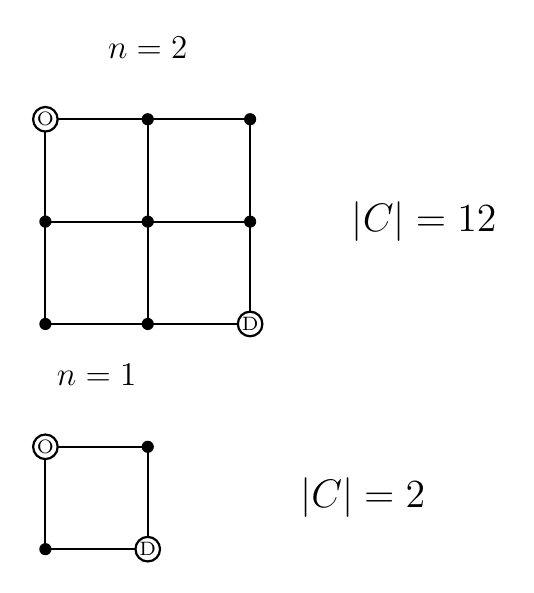
\begin{tikzpicture}[x=1.3cm,y=-1.3cm, line width=0.8pt]

% =========================
% n = 2
% =========================
\begin{scope}[shift={(0,0)}]
  % label
  \node[font=\large] at (1,-0.7) {$n=2$};

  % horizontal edges
  \draw (0,0) -- (1,0) -- (2,0);
  \draw (0,1) -- (1,1) -- (2,1);
  \draw (0,2) -- (1,2) -- (2,2);

  % vertical edges
  \draw (0,0) -- (0,1) -- (0,2);
  \draw (1,0) -- (1,1) -- (1,2);
  \draw (2,0) -- (2,1) -- (2,2);

  % black nodes
  \fill (1,0) circle (2.2pt);
  \fill (2,0) circle (2.2pt);
  \fill (0,1) circle (2.2pt);
  \fill (1,1) circle (2.2pt);
  \fill (2,1) circle (2.2pt);
  \fill (0,2) circle (2.2pt);
  \fill (1,2) circle (2.2pt);

  % O and D
  \draw[fill=white] (0,0) circle (0.12);
  \node at (0,0) {\scriptsize O};

  \draw[fill=white] (2,2) circle (0.12);
  \node at (2,2) {\scriptsize D};

  % |C|
  \node[font=\Large] at (3.7,1) {$|C|=12$};
\end{scope}

% =========================
% n = 1
% =========================
\begin{scope}[shift={(0,3.2)}]
  % label
  \node[font=\large] at (0.5,-0.7) {$n=1$};

  % square
  \draw (0,0) -- (1,0) -- (1,1) -- (0,1) -- (0,0);

  % black nodes
  \fill (1,0) circle (2.2pt);
  \fill (0,1) circle (2.2pt);

  % O and D
  \draw[fill=white] (0,0) circle (0.12);
  \node at (0,0) {\scriptsize O};

  \draw[fill=white] (1,1) circle (0.12);
  \node at (1,1) {\scriptsize D};

  % |C|
  \node[font=\Large] at (3.1,0.5) {$|C|=2$};
\end{scope}

\end{tikzpicture}}
  \caption{Examples of grid networks and the number of simple paths.}
  \label{fig:grid-paths}
\end{figure}

\begin{table}[tb]
\centering
\caption{Number of simple paths in the grid network}
\label{tab:simple-paths}
\begin{tabular}{r r}
\toprule
$n$ & simple paths \\
\midrule
1  & 2 \\
2  & 12 \\
3  & 184 \\
4  & 8,512 \\
5  & 1,262,816 \\
6  & 575,780,564 \\
7  & 789,360,053,252 \\
8  & 3,266,598,486,981,640 \\
9  & 41,044,208,702,632,496,804 \\
10 & 1,568,758,030,464,750,013,214,100 \\
11 & 182,413,291,514,248,049,241,470,885,236 \\
12 & 64,528,039,343,270,018,963,357,185,158,482,118 \\
13 & 69,450,664,761,521,361,664,274,701,548,907,358,996,488 \\
14 & 227,449,714,676,812,739,631,826,459,327,989,863,387,613,323,440 \\
15 & 2,266,745,568,862,672,746,374,567,396,713,098,934,866,324,885,408,319,028 \\
\bottomrule
\end{tabular}
\end{table}


\subsection{動的離散選択モデル}


\subsection{時間構造化ネットワークの導入}


\subsection{摂動効用型経路選択モデル}
動的離散選択モデルとは異なるアプローチで経路非列挙型の経路選択モデルも提案されている．

% 4.1 選択肢集合列挙問題
% 経路は膨大
% 活動系列はさらに膨大
% choice set の定義自体が難しい
% 4.2 列挙型経路選択モデルの限界
% サンプリングバイアス
% 列挙ルール依存
% 観測されない代替経路
% 4.3 Dynamic / Recursiveな表現
% Recursive Logit
% Dynamic decision model
% Perturbed Utility Route Choice
% リンク単位・状態単位での逐次選択

% 4.4 
% 多主体相互作用・時空間制約

% この節はかなり重要です。
% 「交通分野では経路選択を普通のMNLに入れれば済むわけではない」という話が出せるからです。